\documentclass{beamer}
\usepackage{latexsym}
\usepackage{graphicx}
\usetheme{Warsaw}

\title{Chapter 2}
\subtitle{Training Machine Learning Algorithms for Classification}

\begin{document}

\maketitle

\begin{frame}
  \frametitle{Biology}
   \begin{center}
    \begin{figure}
      \includegraphics[width=\textwidth]{Code/ch02/images/02_01.png}
    \end{figure}
   \end{center}
\end{frame}

\begin{frame}
  \frametitle{Logic Gate}
  \begin{center}
    \begin{figure}
      \includegraphics[width=\textwidth]{Code/ch02/images/02_01.png}
    \end{figure}
  \end{center}
  \begin{itemize}
  \item Simple logic gate with binary outputs
  \item Signals arrive at dendrites
  \item Integrated into cell body
  \item If signal exceeds threshold, generate output, and pass to axon
  \end{itemize}
\end{frame}

\begin{frame}
  \frametitle{Rosenblatt Perceptron}
  \begin{itemize}
  \item Binary classification task
  \item Positive class (1) vs. negative class (-1)
  \item Define activation function $\phi(z)$
  \item Takes as input a dot product of input and weights
  \item Net input: $z = w_1 x_1 + \dots + w_m x_m$
  \end{itemize}

  \[
  \mathbf{w} = \begin{bmatrix}
    w^{(1)}  \\
    w^{(2)}  \\
    \vdots  \\
    w^{(m)}
  \end{bmatrix},
  \mathbf{x} = \begin{bmatrix}
    x^{(1)}  \\
    x^{(2)}  \\
    \vdots  \\
    x^{(m)}
  \end{bmatrix}
  \]

\end{frame}

\begin{frame}
  \frametitle{Heaviside step function}
  \begin{itemize}
  \item $\phi(z)$ known as activation
  \item if activation above some threshold, predict class 1
  \item predict class -1 otherwise
  \end{itemize}
  Heaviside Step Function

  \[ \phi(z) = \begin{cases}
    1  & \text{ if } z \ge \theta \\
    -1 & \text{ otherwise }.
  \end{cases}
  \]
\end{frame}

\begin{frame}
\frametitle{Step function simplified}
Bring the threshold $\theta$ to the left side of the equation and define a weight-zero as $w_0 = -\theta$ and $x_0=1$, so that we write $\mathbf{z}$ in a more compact form

\[
z  = w_0 x_0 + w_1 x_1 + \dots + w_m x_m = \mathbf{w^T x}
\]

and

\[ \phi(z) = \begin{cases}
      1  & \text{ if } z \ge 0 \\
      -1 & \text{ otherwise }.
   \end{cases}
\]
\end{frame}

\begin{frame}
  \frametitle{Basic Linear Algebra}
  Vector dot product
  \[
  z  = \mathbf{w^T x} = \sum_{j=0}^{m} \mathbf{w_j} \mathbf{x_j}
  \]

  \[
  \big[1 \quad 2 \quad 3 \big] \times \begin{bmatrix}
    4  \\
    5  \\
    6
  \end{bmatrix} = 1 \times 4 + 2 \times 5 + 3 \times 6 = 32.
  \]
\end{frame}

\begin{frame}
  \frametitle{Input squashed into a binary output}
  \includegraphics[width=\textwidth]{Code/ch02/images/02_02.png}
\end{frame}

\begin{frame}
  \frametitle{Rosenblatt perceptron algorithm}
  \begin{enumerate}
  \item Initialize the weights to 0 or small random numbers.
  \item For each training sample $\mathbf{x}^{(i)}$, perform the following steps:
    \begin{enumerate}
    \item Compute the output value $\hat{y}$.
    \item Update the weights.
    \end{enumerate}
  \end{enumerate}
\end{frame}

\begin{frame}
  \frametitle{Weight update}
  Weight update rule:
  \[
  w_j := w_j + \Delta w_j
  \]
  Perceptron learning rule:
  \[
  \Delta w_j = \eta \bigg( y^{(i)} - \hat{y}^{(i)} \bigg)x_{j}^{(i)}
  \]
  Where $\eta$ is the learning rate (a constant between 0.0 and 1.0), $y^{(i)}$ is the true class label of the $i$th training sample, and $\hat{y}^{(i)}$ is the predicted class label.
\end{frame}

\begin{frame}
  \frametitle{Update rule examples}
  Correct prediction, weights unchanged:
  \[
  \Delta w_j = \eta \bigg( -1 -- 1 \bigg)x_{j}^{(i)} = 0
  \]

  \[
  \Delta w_j = \eta \bigg( 1-1 \bigg)x_{j}^{(i)} = 0
  \]
  Wrong prediction, weights pushed towards the positive or negative class:
  \[
  \Delta w_j = \eta \bigg( 1 -- 1 \bigg)x_{j}^{(i)} = \eta(2)x_{j}^{(i)}
  \]

  \[
  \Delta w_j = \eta \bigg( -1-1 \bigg)x_{j}^{(i)} = \eta(-2)x_{j}^{(i)}
  \]
\end{frame}

\begin{frame}
  \frametitle{Linear separability}
  \includegraphics[width=\textwidth]{Code/ch02/images/02_03.png}
\end{frame}

\begin{frame}
  \frametitle{Convergence}
  Convergence guaranteed if
  \begin{itemize}
  \item The two classess linearly separable
  \item Learning rate is sufficiently small
  \end{itemize}
  If classes cannot be seprated:
  \begin{itemize}
  \item Set a maximum number of passes over the training dataset (epochs)
  \item Set a threshold for the number of tolerated misclassifications
  \item Otherwise, it will never stop updating weights (converge)
  \end{itemize}
\end{frame}

\begin{frame}
  \frametitle{Linear separability}
  \includegraphics[width=\textwidth]{Code/ch02/images/02_04.png}
\end{frame}

\begin{frame}
  \frametitle{Perceptron implementation}
  \href{https://github.com/rasbt/python-machine-learning-book/blob/master/code/ch02/ch02.ipynb}{\beamergotobutton{iPython notebook on github}}
\end{frame}

\begin{frame}
  \frametitle{ADAPtive LInear NEuron (Adaline)}
  \begin{itemize}
  \item Weights updated based on a linear activation function
  \item Remember that perceptron used a unit step function
  \item  $\phi(z)$ is simply the identity function of the net input

    \[
    \phi \big( \mathbf{w}^T \mathbf{x} \big) = \mathbf{w}^T \mathbf{x}
    \]

    \item A quantizer is then used to predict class label
  \end{itemize}
\end{frame}

\begin{frame}
  \frametitle{Adaline: notice the difference with perceptron}
  \includegraphics[width=\textwidth]{Code/ch02/images/02_09.png}
\end{frame}

\begin{frame}
  \frametitle{Cost functions}
  \begin{itemize}
  \item ML algorithms often define an \emph{objective} function
  \item This function is optimized during learning
  \item It is often a \emph{cost} function we want to minimize
  \item Adaline uses a cost function $J(\cdot)$
  \item Learns weights as the sum of squared errors (SSE)
    \[
    J(\mathbf{w}) = \frac{1}{2} \sum_i \bigg(y^{(i)}  - \phi \big(z^{(i)} \big) \bigg)^2
    \]
  \end{itemize}
\end{frame}

\begin{frame}
  \frametitle{Advantages of Adaline cost function}
  \begin{itemize}
  \item The linear activation function is differentiable
  \item Unlike the unit step function
  \item It is convex
  \item Can use \emph{gradient descent} to learn the weights
  \end{itemize}
\end{frame}

\begin{frame}
\frametitle{What is the gradient? Ask Wikipedia:}
\begin{itemize}
\item The gradient is a multi-variable generalization of the derivative. While a derivative can be defined on functions of a single variable, for functions of several variables, the gradient takes its place.
\item Like the derivative, the gradient represents the slope of the tangent of the graph of the function. More precisely, the gradient points in the direction of the greatest rate of increase of the function, and its magnitude is the slope of the graph in that direction.
\end{itemize}
\end{frame}

\begin{frame}
  \frametitle{Gradient Descent}
  \includegraphics[width=\textwidth]{Code/ch02/images/02_10.png}
\end{frame}

\begin{frame}
  \frametitle{Gradient descent: an intuition}
  \begin{itemize}
  \item Suppose you are at the top of a mountain, and you have to reach a lake which is at the lowest point of the mountain (a.k.a valley). A twist is that you are blindfolded and you have zero visibility to see where you are headed. So, what approach will you take to reach the lake?
  \item The best way is to check the ground near you and observe where the land tends to descend. This will give an idea in what direction you should take your first step. If you follow the descending path, it is very likely you would reach the lake.
  \end{itemize}
  \vspace{0.2in}
  \tiny
  https://www.analyticsvidhya.com/blog/2017/03/introduction-to-gradient-descent-algorithm-along-its-variants/
\end{frame}

\begin{frame}
  \frametitle{Gradient Descent: an intuition}
  \center
  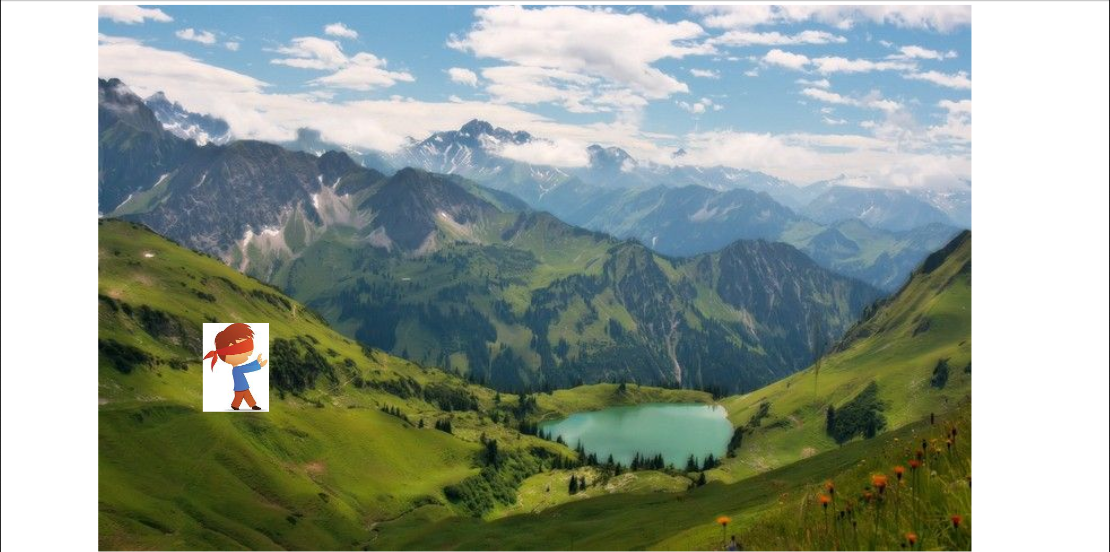
\includegraphics[scale=0.40]{Images/grad_desc1.png}
  \tiny
  \vspace{0.2in}
  https://www.analyticsvidhya.com/blog/2017/03/introduction-to-gradient-descent-algorithm-along-its-variants/
\end{frame}

\begin{frame}
  \frametitle{Gradient Descent: an intuition}
  \center
  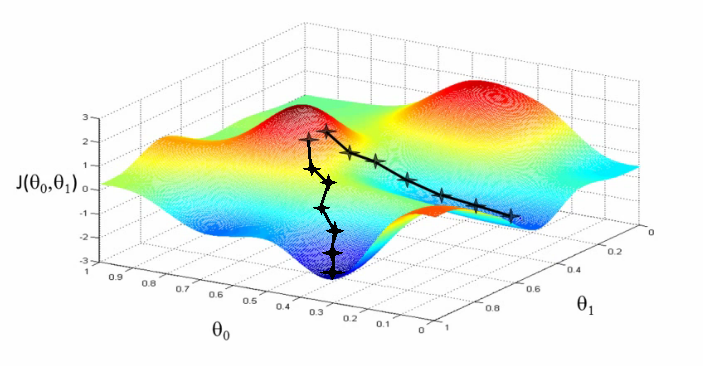
\includegraphics[scale=0.8]{Images/grad_desc2.png}
  \vspace{0.2in}
  \tiny
  https://www.analyticsvidhya.com/blog/2017/03/introduction-to-gradient-descent-algorithm-along-its-variants/
\end{frame}

\begin{frame}
  \frametitle{Gradient Descent}
  \begin{itemize}
  \item Weights updated by taking small steps
  \item Step size determined by learning rate
  \item Take a step away from the gradient $\nabla J(\mathbf{w})$ of the cost function
    \[
    \mathbf{w} := \mathbf{w} + \Delta \mathbf{w}.
    \]
  \item The weight change is defined as follows:
    \[
    \Delta \mathbf{w} = - \eta \nabla J(\mathbf{w})
    \]
  \end{itemize}
\end{frame}

\begin{frame}
  \frametitle{Gradient computation}
  To compute the gradient of the cost function, we need to compute the partial derivative of the cost function with respect to each weight $w_j$,

  \[
  \frac{\partial J}{\partial w_j} = - \sum_i \bigg( y^{(i)} - \phi \big(z^{(i)} \big) \bigg) x_{j}^{(i)},
  \]

  Weight update of weight $w_j$

  \[
  \Delta w_j = - \eta \frac{\partial J}{\partial w_j} = \eta  \sum_i \bigg( y^{(i)} - \phi \big(z^{(i)} \big) \bigg) x_{j}^{(i)}
  \]

  We update all weights simultaneously, so Adaline learning rule becomes

  \[
  \mathbf{w} := \mathbf{w} + \Delta \mathbf{w}.
  \]
\end{frame}

\begin{frame}
  \frametitle{Partial derivatives}
  \begin{equation*}
    \begin{split}
      & \frac{\partial J}{\partial w_j} = \frac{\partial}{\partial w_j} \frac{1}{2} \sum_i \bigg(  y^{(i)} - \phi \big( z^{(i)} \big)  \bigg)^2 \\
      & = \frac{1}{2} \frac{\partial}{\partial w_j} \sum_i \bigg(  y^{(i)} - \phi \big( z^{(i)} \big)  \bigg)^2 \\
      & = \frac{1}{2} \sum_i 2 \big( y^{(i)} - \phi(z^{(i)})\big)  \frac{\partial}{\partial w_j} \Big( y^{(i)}  - \phi({z^{(i)}}) \Big) \\
      & = \sum_i \big( y^{(i)}  - \phi (z^{(i)})   \big) \frac{\partial}{\partial w_j} \Big( y^{(i)} - \sum_i \big(w^{(i)}_{j} x^{(i)}_{j} \big) \Big) \\
      & = \sum_i \bigg(  y^{(i)} - \phi \big( z^{(i)} \big)  \bigg) \bigg( - x_{j}^{(i)} \bigg) \\
      & = - \sum_i \bigg(  y^{(i)} - \phi \big( z^{(i)} \big)  \bigg) x_{j}^{(i)}  \\
    \end{split}
  \end{equation*}
\end{frame}

\begin{frame}
  \frametitle{Adaline learning rule vs. Perceptron rule}
  \begin{itemize}
  \item Looks (almost) identical. What is the difference?
  \item $\phi(z^{(i)})$ with $z^{(i)} = \mathbf{w}^T \mathbf{x}^{(i)}$ is a real number
  \item And not an integer class label as in Perceptron
  \item The weight update is done based on \emph{all} samples in training set
  \item Perceptron updates weights incrementally after each sample
    \item This approach is known as ``batch'' gradient descent
  \end{itemize}
\end{frame}

\begin{frame}
  \frametitle{Perceptron implementation}
  \href{https://github.com/rasbt/python-machine-learning-book/blob/master/code/ch02/ch02.ipynb}{\beamergotobutton{iPython notebook on github}}
\end{frame}

\begin{frame}
  \frametitle{Lessons learned}
  \includegraphics[width=\textwidth]{Code/ch02/images/02_12.png}
  \begin{itemize}
  \item Learning rate too high: error becomes larger (overshoots global min)
  \item Learning rate too low: takes many epochs to converge
    \item Feature normalization
  \end{itemize}
\end{frame}

\begin{frame}
  \frametitle{Stochastic gradient descent (SGD)}
  \begin{itemize}
  \item Large dataset with millions of data points (``big data'')
  \item Batch gradient descent costly
  \item Need to compute the error for the entire dataset ...
  \item ... to take one step towards the global minimum!
    \[
    \Delta \mathbf{w} = \eta \sum_i \bigg( y^{(i)} - \phi \big( z^{(i)}\big) \bigg) \mathbf{x}^{(i)}.
    \]
  \item SGD updates the weights incrementally for each training sample
    \[
    \Delta \mathbf{w} = \eta  \bigg( y^{(i)} - \phi \big( z^{(i)}\big) \bigg) \mathbf{x}^{(i)}.
    \]
  \end{itemize}
\end{frame}

\begin{frame}
  \frametitle{SGD details}
  \begin{itemize}
  \item Approximation of gradient descent
  \item Reaches convergence faster because of frequent weight updates
  \item Important to present data in random order
  \item Learning rate often gradually decreased (adaptive learning rate)
  \item Can be used for online learning
  \item Middle ground between SGD and batch GD is known as \emph{mini-batch learning}
    \begin{itemize}
    \item E.g. 50 examples at a time
    \item Can use vector/matrix operations rather than loops as in SGD
    \item Vectorized operations highly efficient
    \end{itemize}
  \end{itemize}
\end{frame}

\begin{frame}
  \frametitle{}
  \begin{itemize}
  \item
  \end{itemize}
\end{frame}

\end{document}
